\subsection{Krylov Subspace Methods}
\label{sec:krylov_methods}

Even though the methods introduced in the previous chapter are guaranteed to converge, the restriction to a one-dimensional search space severely limits the progress they can achieve in a single iteration. Thus they might require a large number of iterations before they produce an accurate approximation of the desired solution. As a natural extension, faster progress could be expected from a larger search-space by minimizing the residual over multiple dimensions at the same time. Simultaneously, the search-space has to remain small enough in order to obtain a fast solution to the minimization process. Since there is a trade-off between them minimization cost and the number of iterations, an intuitive solution would be to create a sequence of subspaces $S$ with increasing dimensions such that:
\begin{equation}
    S_1 \subset \ S_2 \subset S_3 \subset \dots
\end{equation}

\noindent At each iteration $k$ of the iterative solver, the subspace $S_k$ satisfying $dim(S_k)=k$ is searched for a solution $\hat{x}$ that minimizes:
\begin{equation}
\label{eqn:residual}
    f(x)= r = Ax-b
\end{equation}

\noindent Note that because $S_n=\real$, this sequence will ultimately produce the exact solution to the problem (in absence of rounding errors). However, since this would amount to more work than just solving the system directly, a good approximation should be achieved in $k$ iterations with $k \ll n$. Hence the challenge is to find such a subspace sequence that minimizes $r$ in the most optimal way. As illustrated in the one-dimensional case, the error of the approximation decreases most rapidly in the direction of the residual. Consequently it seems reasonable to choose $S_{k+1}$ at iteration $k$ so that it includes both $\iter[k]{x}$ and $\iter[k]{r}$, which guarantees that the update $\iter[k+1]{x}$ will be at least as good as the one-dimensional case \cite{golub_matrix_2013}. From $\iter[0]{x}$ as the initial guess and Equation~\hyperref[eqn:residual]{\ref{eqn:residual}} it follows that $\iter[k]{r} \in span\{\iter[k]{x},A\iter[k]{x}\}$ and the only way to satisfy this requirement is:
\begin{equation}
    S_k=\mathcal{K}(A,\iter[0]{r}, k) = span\{\iter[0]{r}, A\iter[0]{r}, A^2\iter[0]{r},\dots A^{k-1}\iter[0]{r}\}
\end{equation}

\noindent This kind of sequence is referred to as a Kryolov subspace and viewed from the angle of polynomial approximation, a vector $v$ in such a Krylov subspace can be expressed in general terms as a linear combination of powers of $A$ times $y$:
\begin{equation}
\label{eqn:poly1}
    v = c_0y+c_1Ay+c_2A^2y+\dots+c_{m-1}A^{m-1}y
\end{equation}

\noindent In other words $v$ is a polynomial in $A$ times $y$ and by defining $p$ as a polynomial of the form $p(z) = c_0+c_qz+c_2z^2+\dots+c_{m-1}z^{m-1}$, the following, compact description can be achieved:
\begin{equation}
\label{eqn:poly2}
v=p(A)y  
\end{equation}

\noindent A Krylov subspace method for solving a linear system will thus attempt to improve a initial solution $\iter[0]{x}$ based on the residual $\iter[0]{r} = b-A\iter[0]{x}$ by updating it with such a vector $v \in \mathcal{K}(A, \iter[0]{r},k)$, which corresponds to:
\begin{equation}
    A^{-1}b \approx \iter{x} = \iter[0]{x}+p(A)\iter[o]{r}
\end{equation}

\noindent From this point going forward, $\mathcal{K}(A, \iter[0]{r},k)$ will be simply denoted as $\mathcal{K}_k$ if there is no ambiguity. Furthermore, note that even though all Krylov subspace based techniques provide the same type of polynomial approximation, they differ in the constraints $\mathcal{L}_k$ used to build these approximation, giving rise to a number of distinct algorithm (see \cite{saad_iterative_2003} for a comprehensive overview) and only a subset will be discussed in this research.



\subsubsection{Conjugate Gradient (CG)}
\label{sec:conjugate_gradient}

The easiest way to interpret the conjugated gradient method (first proposed by \cite{hestenes_methods_1952} is as an extension of the steepest descent algorithm to Krylov subspaces. Indeed, since in the first iteration, the Krylov subspace $\mathcal{K}_1=\{\iter[0]{r}\}$, the initial steps taken by the two algorithms are exactly equivalent. However, for CG the projection subspace extends in the second iteration to $\mathcal{K}_2=\{\iter[0]{r}, A\iter[0]{r}\}$ (a two-dimensional space), while it remains one dimensional for steepest descent. In other words, both methods optimize the error $\iter[0]{d}$ in the first step along the residual vector $\iter[0]{r}$ (i.e. the search direction $\iter[0]{p}=\iter[0]{r}$), but they differ in the second step. While steepest descent minimizes the new error $\iter[1]{d}$ only along the new residual $\iter[r]{1}$ (i.e. $\iter[1]{p}=\iter[1]{r}$, CG minimizes the error for the whole plane spanned by $span\{\iter[0]{r}, \iter[1]{r}\}$. This can be achieved by selecting a new search direction $\iter[1]{p}$ that is $A$-orthogonal to all previous ones \cite{trefethen_numerical_1997}. If the bases of the Krylov subspace are rewritten as:
\begin{equation}
    \mathcal{K}_k = span\{\iter[0]{r}, A\iter[0]{r}, \dots A^{k-1}\iter[0]{r}\} = span\{q_0, q_1, \dots q_{k-1}\}
\end{equation}

\noindent Then this corresponds to the condition $q_i \perp q_j$ with $i\neq j$ for all $i$,$j$ from $0$ to $k$. As a result, the algorithm introduced by \cite{hestenes_methods_1952} requires two modifications when compared to steepest descent.
\begin{enumerate}
    \item Introduce a vector $p$ ($\iter[0]{p} = \iter[0]{r}$) representing the search direction.
    \item Determine the new search direction $\iter[k+1]{p}$ so that it is $A$-orthogonal to all previous ones (or, equivalently create an orthogonal basis $q_{k}$ for the Krylov subspace $\mathcal{K}_{k+1}$).
\end{enumerate}

\begin{algorithm}[h]
  \caption{Conjugate Gradient}
  \label{alg:conjugate_gradient}
  \SetAlgoLined
  \DontPrintSemicolon
  \KwIn{matrix $A \in \mathbb{R}^{n \times n}$, vector $b \in \mathbb{R}^{n}$ and initial solution $\iter[0]{x} \in \mathbb{R}^{n}$}
  \KwOut{approximate solution $\iter[m]{x}$ to the system $Ax=b$\\
  \hrulealg}
  $\iter[0]{r} = b-A\iter[0]{x}$ \\
  $p = \iter[0]{r}$ \\
  \For{$i = 1$ \KwTo $m$} {
    $\alpha = \langle \iter[i-1]{r};\iter[i-1]{r} \rangle / \langle Ap;p \rangle$ \\
    $\iter[i]{x} = \iter[i-1]{x}+\alpha p$ \\
    $\iter[i]{r} = \iter[i-1]{r} - \alpha Ap$ \\
    $\beta = \langle \iter[i]{r};\iter[i]{r} \rangle / \langle \iter[i-1]{r};\iter[i-1]{r} \rangle$ \\
    $p = \iter[i]{r} + \beta p$ \\
  }
\end{algorithm}

\noindent The pseudo-code provided in Algorithm~\hyperref[alg:conjugate_gradient]{\ref{alg:conjugate_gradient}} implements those changes. The modifications in line 1 correspond to the requierement that the new residual needs to be orthogonal to the Krylov subspace $\mathcal{K}_k$ (instead of just the previous residual), using a little simplification in the numerator of the fraction. Because $p$ is built as a linear combination of the previous residuals, $\langle \iter[i]{r};\iter[i]{r} \rangle = \langle \iter[i]{r};\iter[i]{p} \rangle$ is valid and the terms can be used interchangeably. The addition of lines 7 \& 8 corresponds to the Gram-Schmidt orthogonalization of the basis vectors, ensuring that the new search direction is $A$-orthogonal to all previous ones. Note that since $\iter[k]{p}$ is already $A$-orthogonal to all $\iter[i]{p}, i=0,\dots,k-1$, the only orthogonalization that is needed for $\iter[k+1]{p}$ is with respect to $\iter[k]{p}$. In other words, we have the following identities of subspaces:
\begin{equation}
  \begin{aligned}
    \mathcal{K}_k 
    & =\langle \iter[1]{x}, \iter[2]{x}, \dots \iter[k]{x} \rangle 
   & & = \langle \iter[0]{p}, \iter[1]{p}, \dots \iter[k-1]{p} \rangle \\
    & = \langle \iter[0]{r}, \iter[1]{r}, \dots \iter[k-1]{r} \rangle
   & & =\langle \iter[0]{r}, A\iter[0]{r}, \dots A^{k-1}\iter[0]{r}\rangle\\
  \end{aligned}
\end{equation}

\noindent Furthermore, for those subspaces, the following properties hold:
\begin{equation}
    \langle\iter[i]{r};\iter[j]{r}\rangle =0 \;\; \text{ and } \;\; \langle\iter[i]{p};\iter[j]{p}\rangle_A =0
    \;\; \text{ for all }\;\; i,j <k, i \neq j
\end{equation}

\noindent Since all Krylov subspace iterations can be analyzed in terms of matrix polynomials (see Equations~\hyperref[eqn:poly1]{\ref{eqn:poly1}} \& \hyperref[eqn:poly2]{\ref{eqn:poly2}}), the same is true for the CG method. By defining $P_k$ as the set of polynomials $q$ of degree $\leq k$ with $q(0)=1$ and $d$ denoting the initial error $\iter[0]{d} = x^*-\iter[0]{x}$ the problem CG tries to solve can be reformulated as finding the polynomial $q_k$ such that:
\begin{equation}
    p_k = \underset{p\in P_k}{min} \norm{p_k(A)\iter[0]{d}}_A
\end{equation}

\noindent In terms of convergence of the CG method, it is known that the speed depends on the location of the spectrum of $A$ and \cite{trefethen_numerical_1997} expressed the two best known corollaries in the following form:
\begin{itemize}
    \item CG converges in at most $m$ steps, if $A$ has exactly $m$ distinct eigenvalues
    \item If the condition number $\kappa_2(A) $ is not too large, convergence can be expected in $\mathcal{O}(\sqrt{\kappa_2(A})$ iterations because the following is known for the error $d$:
\begin{equation}
        \frac{\norm{\iter[k]{d}}_A}{\norm{\iter[0]{d}}_A} \leq 2 \left( \frac{\sqrt{\kappa_2(A)}-1}{\sqrt{\kappa_2(A)}+1}\right)^k
\end{equation}
\end{itemize}

\noindent Finally, it should be noted that the formulation in Algorithm~\hyperref[alg:conjugate_gradient]{\ref{alg:conjugate_gradient}} is the one originally proposed by \cite{hestenes_methods_1952}, but several other alternative variants are possible. The key point is the construction of the orthogonal bases for the Krylov subspace $\mathcal{K}_k$ and depending on how those are obtained (e.g. the orthogonalization scheme employed) the denotations of the algorithms deviate slightly. Due to the importance of this part for all Krylov subspace based iterative methods, the two main techniques for obtaining such bases will be discussed in the next sections.


\subsubsection{Arnolid's method}
\label{sec:arnoldi}
This method, first proposed by Arnoldi \cite{arnoldi_principle_1951} enforces the Galerkin condition $A\iter[k]{x} -b \perp \mathcal{K}_k$ onto the constructed Krylov subspace and is applicable to general non-Hermitian matrices. It was originally proposed for the purpose of reducing a dense matrix into Hessenberg from via a unitary transformation. But at its core, it is an algorithm for building an orthogonal basis of the Krylov subspace $\mathcal{K}_k$. It was later discovered that it is also an efficient technique for eigenvalue approximation, and was then extended to the solution of linear systems \cite{saad_iterative_2003}. 

\begin{algorithm}[h]
  \caption{Arnoldi's Method}
  \label{alg:arnoldi}
  \SetAlgoLined
  \KwIn{non-singular matrix $A \in \mathbb{R}^{n \times n}$, arbitrary vector $y \in \mathbb{R}^{n}$}
  \KwOut{\\ Hessenberg matrix $H \in \mathbb{R}^{(m+1) \times m}$ \\
  sequence of orthonormal vectors $\iter[i]{q}\in \mathbb{R}^{n}$ where $i = 1, 2, \dots, k$\\
  \hrulealg}
  $\iter[1]{q}= y\:/\norm{y}_2$ \\
  \For{$i = 1$ \KwTo $k$} {
    $w =A\cdot \iter[i]{q}$ \\
    \For{$j = 1$ \KwTo $i$} {
      $h_{j,i} = w^T\cdot \iter[j]{q}$ \\
      $ w = w - h_{j,i}\cdot \iter[j]{q}$}
    $h_{i-1,i} = \norm{w}_2$ \\
    \If{$h_{i-1,i} = 0$}{\Return}
    $\iter[i-1]{q} = w/h_{i+1,i}$
  }
\end{algorithm}

\noindent Following the process outlined in Algorithm~\hyperref[alg:arnoldi]{\ref{alg:arnoldi}}, the successive iterates are related by the following formula:
\begin{equation}
\label{eqn:arnoldi}
AQ_k=Q_{k+1}\tilde{H}_k
\end{equation}
\noindent where $\tilde{H}_k$ is the $(k+1) \times k$ upper-left section of $H$ (and thus also a Hessenberg matrix) and $Q_k$ is:
\begin{equation}
  Q_k =
  \left[
    \begin{array}{c|c|c}
      & & \\
      \iter[1]{q} &\dots & \iter[k]{q} \\
      & & \\
    \end{array}
  \right] 
\end{equation}

\noindent This is equivalent to:

\begin{equation}
  \left[
    \begin{array}{ccc}
      &  & \\
      & A & \\
      &  & \\
    \end{array}
  \right] \cdot
  \left[
    \begin{array}{c|c|c}
      & & \\
      \iter[1]{q} &\dots & \iter[k]{q} \\
      & & \\
    \end{array}
  \right] = 
  \left[
    \begin{array}{c|c|c}
      & & \\
      \iter[1]{q} &\dots & \iter[k+1]{q} \\
      & & \\
    \end{array}
  \right]
  \left[
    \begin{array}{ccc}
      h_{1,1} & \dots & h_{1,k} \\
      h_{2,1} & \dots &  h_{2,k}\\
      & \ddots & \vdots \\
      & & h_{k+1, k}  \\
    \end{array}
  \right] 
\end{equation}

\noindent Therefore, the $k$-th column of this equation can be denoted as:
\begin{equation}
    A \cdot \iter[k]{q} = h_{1,k}\cdot \iter[1]{q}+ \cdots + h_{k,k}\cdot \iter[k]{q} + h_{k+1,k}\cdot \iter[k+1]{q}
\end{equation}

\noindent From this, it is evident that the vectors $q^i$ form orthonormal bases of the successive Krylov subspaces generated by $A$ and $y$:
\begin{equation}
\label{eqn:krylov_space}
    \mathcal{K}_k=\langle y, Ay, \dots , A^{k-1}y\rangle = \langle \iter[1]{q},\iter[1]{q}, \dots , \iter[1]{k}\rangle
\end{equation}

\noindent Since Krylov subspace iterations can be analyzed in terms of matrix polynomials (see Equations~\hyperref[eqn:poly1]{\ref{eqn:poly1}} \& \hyperref[eqn:poly2]{\ref{eqn:poly2}}), the same is true for Arnoldi's method. By defining 
\begin{equation}
\label{eqn:arnoldi_poly}
    P^n = \{\text{monic polynomials of degree }m\}\text{,}
\end{equation}

\noindent that is all polynomials where the coefficient of the term of degree $m$ is 1 and $p \in P^m$, the vector from Equation~\hyperref[eqn:poly2]{\ref{eqn:poly2}} can be written as $p(A)y=A^my-Q_mz$ for some $z \in \mathbb{R}^m$. Due to the orthogonality condition $p^m(A)y \perp \mathcal{K}_m$, Arnoldi's method has the remarkable property that it finds $z$ such that $\norm{A^my-Q_mz}_2$ is minimal. In other words, it solves the least squares polynomial approximation problem $\norm{p^m(A)y}_2 =$ minimum. The full proof behind this characteristic can be obtained from \cite{trefethen_numerical_1997}, but the general intuition is outlined in Figure~\hyperref[fig:arnoldi]{\ref{fig:arnoldi}}.

\begin{figure}[h]
    \centering
    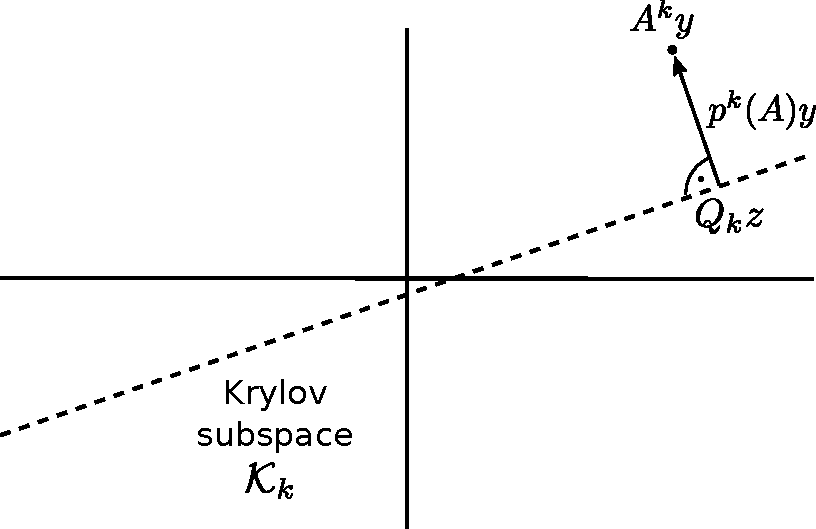
\includegraphics[width=0.6\linewidth]{figures/Arnoldi.pdf}
    \caption{The least squares polynomial approximation problem underlying the Arnoldi iteration as described in \cite{trefethen_numerical_1997}}.
    \label{fig:arnoldi}
\end{figure}

\noindent A final remark on Arnoldi's method has to be made with regards to numerical stability. As can be seen from the pseudo-code given in Algorithm~\hyperref[alg:arnoldi]{\ref{alg:arnoldi}}, the method needs to orthonormalize the resulting vector $w$ against all previous $q^j$'s in each iteration. While several methods are known to achieve this outcome, they differ in terms of speed and numerical stability (for a discussion of the different methods, see \cite{golub_matrix_2013} or \cite{trefethen_numerical_1997}). Algorithm~\hyperref[alg:arnoldi]{\ref{alg:arnoldi}} used the Modified-Gram-Schmidt method, but in principle, any other orthonormalization technique can be incorporated into the method. Variants using ordinary Gram-Schmidt or Householder orthogonalization can be obtained from \cite{saad_iterative_2003}.